\section{Filtros aplicados al flujo de predicciones}
\label{sec:filtrosFlujoPredicciones}

\subsection{Filtros de decisión}
\label{subsec:filtros_decision}

El objetivo principal de estos ``filtros de decisión'' es hacer más consistente el flujo de predicciones que se recibe del modelo. Esto se puede conseguir de distintas formas, entre ellas: reducir la cantidad de predicciones agrupándolas, usar mecanismos para ignorar \textit{outliers} (predicciones que se salen de lo ``normal'' en ese periodo temporal), suavizando los cambios de una predicción a otra (eliminando saltos).

Se plantearon y testearon varias opciones:

\begin{itemize}
    \item \textbf{Filtro por mayoría}: Consiste en, dentro de una ventana de tiempo determinado (el último segundo, los últimos 4 segundos\dots), contar el número de veces que se ha recibido la predicción ``derecha'' y cuántas veces se ha predicho ``izquierda''. La decisión final se obtiene seleccionando la clase con mayor frecuencia de aparición en la ventana seleccionada. Este método proporciona una estrategia sencilla frente a predicciones aisladas erróneas.
    \item \textbf{\textit{Score} ponderado}:  Para cada predicción generada por el modelo, se calcula un valor de confianza a partir de la diferencia absoluta entre las probabilidades asociadas a ambas clases dentro de la ventana temporal:
    \[\textit{Score} = \left|P_{\text{derecha}} - P_{\text{izquierda}}\right|.\]
    Cuanto mayor sea dicha diferencia, mayor será la confianza atribuida a la predicción. Posteriormente, cada predicción se pondera según este \textit{score}, asignando valores positivos a una clase (\textit{right\_hand}) y negativos a la otra (\textit{left\_hand}). Todo esto se hace con el objetivo de obtener una media ponderada que tenga en cuenta tanto la dirección predicha como la seguridad del modelo.
    \item \textbf{Media de probabilidades}: Con este método se promedian independientemente las probabilidades asociadas a cada clase obtenidas en todas las predicciones de una ventana temporal determinada. La decisión final corresponde a la clase cuya probabilidad media resulte mayor. Este enfoque permite aprovechar directamente la información probabilística proporcionada por el modelo y trata de mejorar el método de la mayoría.
    \item \textbf{Filtro con fuga}: Este se basa en un mecanismo acumulativo inspirado en sistemas dinámicos con disminución temporal que no de depende de una ventana temporal. A partir de cada predicción se incrementa un acumulador asociado a la clase correspondiente. De forma periódica, el valor acumulado disminuye mediante un factor de fuga. Cuando el acumulador de una clase supera un determinado umbral, se genera la decisión correspondiente.
    \item \textbf{Suavizado exponencial}: Este método aplica un filtrado temporal recursivo sobre las probabilidades generadas por el modelo, combinando la predicción actual con el histórico de predicciones anteriores sin depender de una ventana de predicciones~\cite{perdikis2011evidence}. Para ello, se calcula una media exponencialmente ponderada en la que las observaciones más recientes tienen un mayor peso que las más antiguas. El grado de influencia de las nuevas predicciones se controla mediante un parámetro de suavizado $\alpha$, a mayor sea este parámetro menos se tendrá en cuenta la nueva predicción y mas la predicción suavizada previa. De esta forma, el sistema reduce fluctuaciones bruscas y variaciones instantáneas provocadas por posibles errores o estados transitorios de las predicciones del modelo, manteniendo al mismo tiempo capacidad de adaptación frente a cambios sostenidos en la intención del usuario. La decisión final se obtiene seleccionando la clase cuya probabilidad suavizada supere un determinado umbral pasado como parámetro.
    Se calcula la probabilidad suavizada para cada clase,siendo $P_{t-1}$ la probabilidad suavizada en el instante $t$, y $p_t$ la probabilidad cruda generada por el modelo en ese mismo instante, la fórmula de actualización es:
    \[P_t = \alpha \cdot P_{t-1} + (1 - \alpha) \cdot p_t.\]
    Este método se mostró especialmente efectivo para mejorar la estabilidad de las predicciones en tiempo real, proporcionando una experiencia de usuario más fluida,consistente y menos inestable a costa de añadir un ligero retardo.
\end{itemize}


\begin{figure}[h]
    \centering
    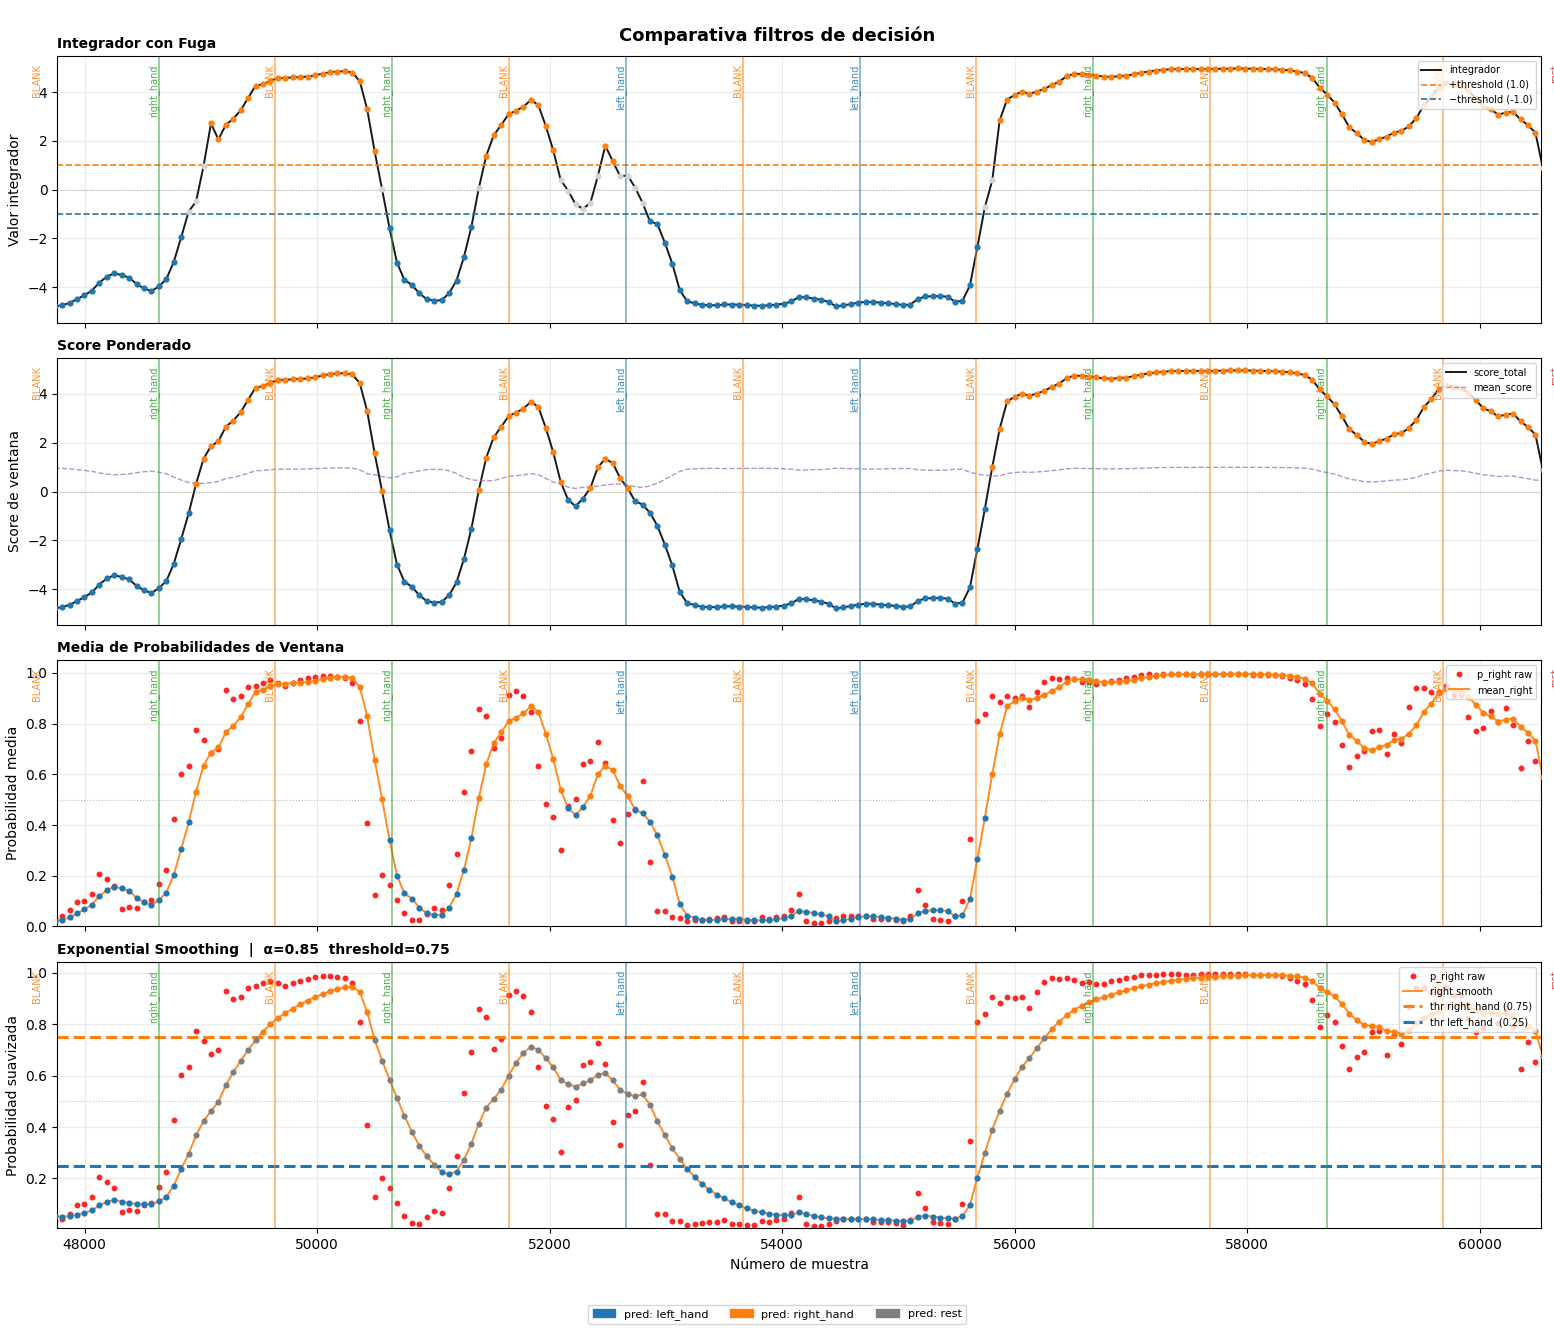
\includegraphics[width=1\textwidth]{Imagenes/Bitmap/comparativa_filtros_decision.png}
    \caption{Comparativa de los cuatro filtros de decisión evaluados sobre una grabación simulada en tiempo real. Los puntos rojos representan las probabilidades crudas generadas por el MIRepNet; los puntos azules, naranjas y grises indican la salida de cada filtro de decisión, correspondiendo a las predicciones de mano izquierda, mano derecha y ninguna clase, respectivamente. Las líneas verticales marcan los instantes en los que se le pidió al usuario que imaginase una determinada acción. Los filtros de Score Ponderado y Media de Probabilidades operan sobre una ventana deslizante de 5 predicciones (aproximadamente 1~segundo), por lo que su salida depende del conjunto de predicciones acumuladas en dicha ventana; en cambio, el Integrador con Fuga y el Alisado Exponencial actualizan su estado con cada nueva predicción de forma incremental, sin depender de una ventana fija. Para el Alisado Exponencial y la Media de Probabilidades se representa únicamente la probabilidad suavizada de la clase derecha, dado que la clase izquierda es su complemento ($1 - p_\text{derecha}$). El Score Ponderado y el Integrador con Fuga producen valores en el rango $[-5,\,5]$. El Alisado Exponencial ofrece una respuesta considerablemente más estable y menos oscilatoria que el resto, a costa de introducir un ligero retardo.}
    \label{fig:comparativa_filtros_decision}
\end{figure}

Para la comparativa de filtros, no se tuvo en cuenta la primera propuesta de filtro por mayoría, ya que se consideró que, aunque es un método sencillo y efectivo para reducir cierto ruido, no aportaba información sobre las probabilidades de las predicciones dentro de la ventana y por lo tanto se pierde información relevante para la posterior fase de juego.

En la Figura~\ref{fig:comparativa_filtros_decision} se muestra una comparativa visual de los cuatro filtros sobre una grabación simulada en tiempo real. El filtro seleccionado para su integración en el sistema fue el suavizado exponencial, debido a su capacidad para mejorar la estabilidad de las predicciones, no depender de un tamaño de ventana deslizante de predicciones y no introducir un retardo excesivo, lo que resultaba especialmente importante para la jugabilidad de los juegos diseñados para el experimento.

El siguiente paso consistió en buscar el mejor valor para el parámetro de suavizado $\alpha$. Para ello, se realizaron pruebas con diferentes valores de $\alpha$ sobre grabaciones simuladas en tiempo real, analizando la respuesta del sistema y la estabilidad de las predicciones, tal y como se muestra en la Figura~\ref{fig:comparativa_parametros_es}. Finalmente, se seleccionó un valor de $\alpha$ = 0,85 y umbral de 0,75 ya que se consideró un buen punto de partida para las pruebas experimentales con participantes.


\begin{figure}[h]
    \centering
    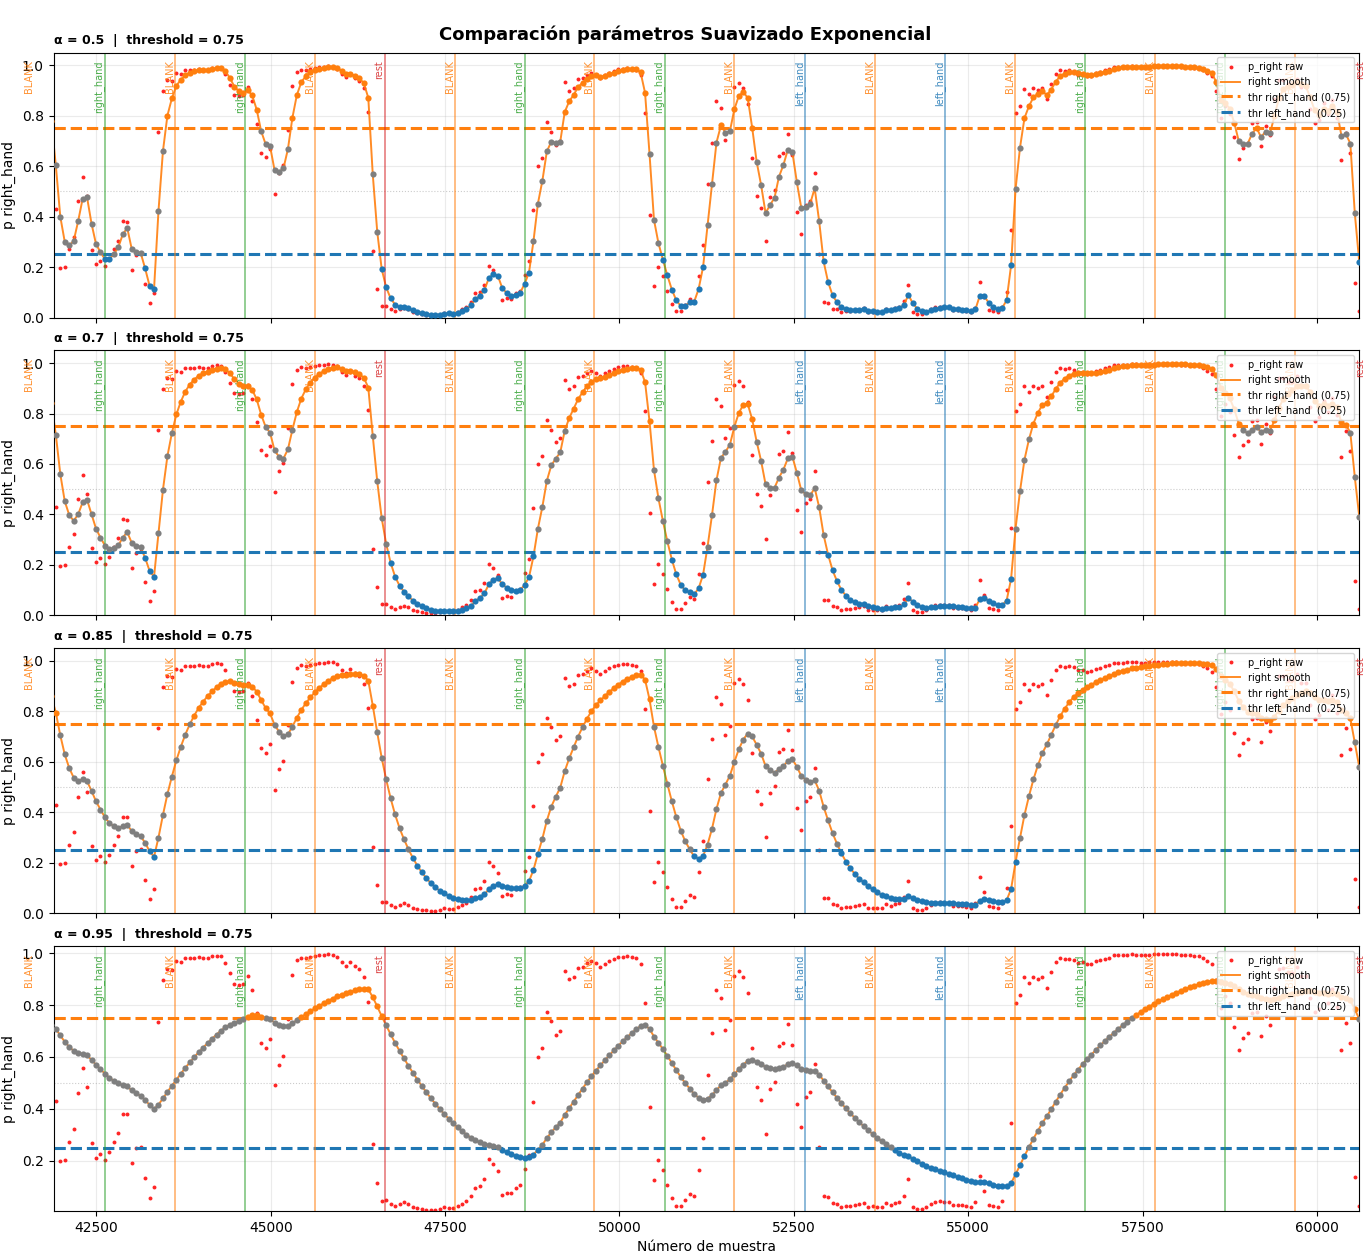
\includegraphics[width=1\textwidth]{Imagenes/Bitmap/ES_comparativa.png}
    \caption{En esta gráfica se compara el desempeño del filtro de Alisado exponencial con diferentes parámetros de suavizado $\alpha$ con el mismo umbral de decisión 0.75, sobre una grabación simulada en tiempo real. Se puede observar que a medida que se incrementa el valor de $\alpha$, la curva de probabilidades suavizadas se vuelve más estable y menos oscilatoria, aunque también introduce un retardo mayor respecto a las probabilidades crudas. Por otro lado un valor cada vez menor de alpha ofrece una respuesta del sistema mas rápida pero también mas inestable, con oscilaciones bruscas que podrían resultar molestas para el usuario. El valor seleccionado de $\alpha$ = 0,85 se considera un buen compromiso entre estabilidad y capacidad de respuesta para las primeras pruebas experimentales.}
    \label{fig:comparativa_parametros_es}
\end{figure}

\subsection{Filtros de ayuda integrados en los juegos}
\label{subsec:filtros_ayuda}

Como ha sido mencionado anteriormente, se diseñaron mecanismos de ayuda para cada juego que permiten reducir los fallos causados por las señales EEG, el sistema o el propio usuario haciendo \textit{motor imagery}. Estos mecanismos, al depender directamente del estado del juego y de las normas del mismo, fueron implementados directamente en el \textit{script} de cada juego. 

El planteamiento seguido fue el siguiente:

\begin{enumerate}
    \item Se diseñó una solución óptima capaz de decidir para cada instante una solución que evite perder.
    \item Se adaptó la solución para que, en vez de tomar la decisión directamente, tuviera en cuenta la salida del modelo: en base a una constante definida (``SEVERIDAD\_AIMBOT'') la ayuda decide si actuar siguiendo la predicción, o corregir la acción.
    \item Se modificó la ayuda ya que, en los casos que se usaba con su severidad al máximo (``SEVERIDAD\_AIMBOT'' = 1, no teniendo en cuenta las predicciones del modelo), resultaba excesivamente antinatural y notorio. La modificación implicó dejar márgen desde que el \textit{aimbot} ``ve'' qué acción debería realizar hasta que realmente la hace. 
\end{enumerate}

Las estrategias resultantes fueron:

\begin{itemize}
    \item \textbf{Ayuda \textit{Wave Runner}}: La implementación de la asistencia en este juego se basa en un cálculo geométrico que evalúa el nivel de peligro de la nave para cada instante. El algoritmo exacto se divide en:
    \begin{enumerate}
        \item \textbf{Cálculo de los límites laterales:} En cada \textit{frame}, el sistema identifica el segmento del túnel en el que se encuentra la nave exactamente (basándose en su coordenada Y, que es fija). Calcula los bordes izquierdo (\textit{left\_bound}) y derecho (\textit{right\_bound}) disponibles en esa altura.
        \item \textbf{División del espacio:} A partir de los bordes calculados, se obtiene el centro ideal del túnel para esa Y concreta. El espacio disponible se divide manteniendo un margen alrededor del centro (\textit{tunnel\_center\_left} y \textit{tunnel\_center\_right}). Si la nave navega dentro de esta porción central, el sistema lo considera zona segura y mantiene el rumbo. Esta división se realizó con el objetivo conseguir que el \textit{aimbot} resulte natural.
        \item \textbf{Cálculo dinámico del umbral:} Cuando la nave se sale de la porción central y se acerca a una de las paredes, se calcula el umbral. El algoritmo lo calcula en base a la constante de severidad (\texttt{SEVERIDAD\_AIMBOT}) y en base a la distancia al borde. Se calcula la distancia de la nave al borde más cercano y se pondera de forma que cuanto más cerca esté del peligro, más alto será el umbral. El umbral resultante será como mínimo \texttt{SEVERIDAD\_AIMBOT - 1}.
        \item \textbf{Decisión e intervención:} Como ya se ha mencionado, la ayuda no actua de forma estricta, compara el umbral dinámico con las probabilidades suavizadas que emite el modelo de IA (como \texttt{p\_right\_smooth}). Por ejemplo, si la nave está a punto de chocar por la izquierda y la probabilidad suavizada de ir a la derecha supera el umbral dinámico exigido, la ayuda toma la acción de ir a la derecha. En caso contrario, se respeta la predicción cruda del usuario (\texttt{string\_to\_action}).
    \end{enumerate}
    De esta forma, se logra el objetivo del diseño: el \textit{aimbot} no actúa de forma intrusiva, sino que suaviza la jugabilidad dejando margen de reacción que varía en función de cuán crítica sea la situación y de la severidad especificada.
    \item \textbf{Ayuda \textit{Project Arrows}}: La ayuda para este segundo juego se centra en la evaluación de la amenaza más cercana. El algoritmo procesa el estado del juego siguiendo estos pasos:
    \begin{itemize}
        \item \textbf{Identificación de la amenaza principal:} En cada llamada, el sistema evalúa todas las flechas enemigas activas en pantalla y calcula su distancia respecto al centro del jugador (\textit{CENTER\_X}). Esto permite aislar y seleccionar únicamente la flecha enemiga más cercana, priorizando el peligro más inmediato.
        \item \textbf{División del espacio:} Igual que en el anterior caso, se toman medidas para evitar que la ayuda actúe de forma prematura y vuelva el juego excesivamente automatizado. El sistema solo contempla la posibilidad de intervenir si la amenaza más cercana ha sobrepasado un límite específico.
        \item \textbf{Umbral e intervención:} A diferencia del cálculo dinámico tratado anteriormente, aquí se establece un umbral de intervención directo basado en la constante de configuración (\texttt{SEVERIDAD\_AIMBOT}). Si la amenaza cruza la zona crítica, la asistencia comprueba las probabilidades del modelo. Si, por ejemplo, el impacto inminente proviene de la izquierda y la probabilidad suavizada de ir hacia la izquierda (\texttt{p\_left\_smooth}) es mayor o igual que el umbral, el sistema asume la intención del usuario e impone la acción de bloqueo. Si el umbral no se alcanza, la asistencia no interviene y se ejecuta la predicción cruda del modelo (\texttt{string\_to\_action}).
    \end{itemize}
    Con esta estrategia, se permite que el jugador tenga tiempo de ver la amenaza, identificarla y reaccionar en consecuencia.
\end{itemize}